\documentclass[6pt]{../../shared/AiTex}

\title{Memoria entrega 4}
\author{A.L.K.}
\date{Abril 2024}

\begin{document}
%\datos{facultad}{universidad}{grado}{asignatura}{subtitulo}{autor}{curso}
\datos{Informática}{Universidad Complutense de Madrid}{Ingeniería informática}{Aprendizaje Automatico y Big Data}{Entrega 6: diseño de redes neuronales}{Alejandro Barrachina Argudo}{2023-2024}
% \portadaApuntes
% \pagestyle{empty}
% \tableofcontents
% \pagestyle{empty}
\justify

\begin{center}

    {\huge \textbf{\underline{\subtitulo}}} \\
    { \lesson - \autor}

\end{center}


\section*{Introducción}

En este documento se explicará el código del entregable 6B y el proceso de diseño de redes neuronales con \textit{pytorch}.

Para esta práctica se usarán los siguientes \textit{imports} vistos en la figura \ref{fig:imports}. Parte del código se reutiliza de la práctica anterior.
\begin{figure}[H]
    \centering
    \lstinputlisting[firstline=1,lastline=11, style=custompython]{../evaluation.py}
    \caption{Código de las bibliotecas usadas}
    \label{fig:imports}
\end{figure}

También usaremos una serie de constantes para todo el programa (figura \ref{fig:constants}).

\begin{figure}[H]
    \centering
    \lstinputlisting[firstline=13,lastline=22, style=custompython]{../evaluation.py}
    \caption{Constantes del programa}
    \label{fig:constants}
\end{figure}

El \textit{dataset} para esta práctica lo generamos aleatoriamente con la función \textit{generate\_data} (figura \ref{fig:generate_data}). El dataset se compone de una linea de datos ``ideales'' y datos con ruido para comprobar la eficacia de la red neuronal. Estos datos se componen en la función \textit{generate\_data\_driver} (figura \ref{fig:generate_data_driver}).

Para dibujar estos datos usaremos la función \textit{plot\_data} (figura \ref{fig:plot_data}).

\begin{figure}[H]
    \centering
    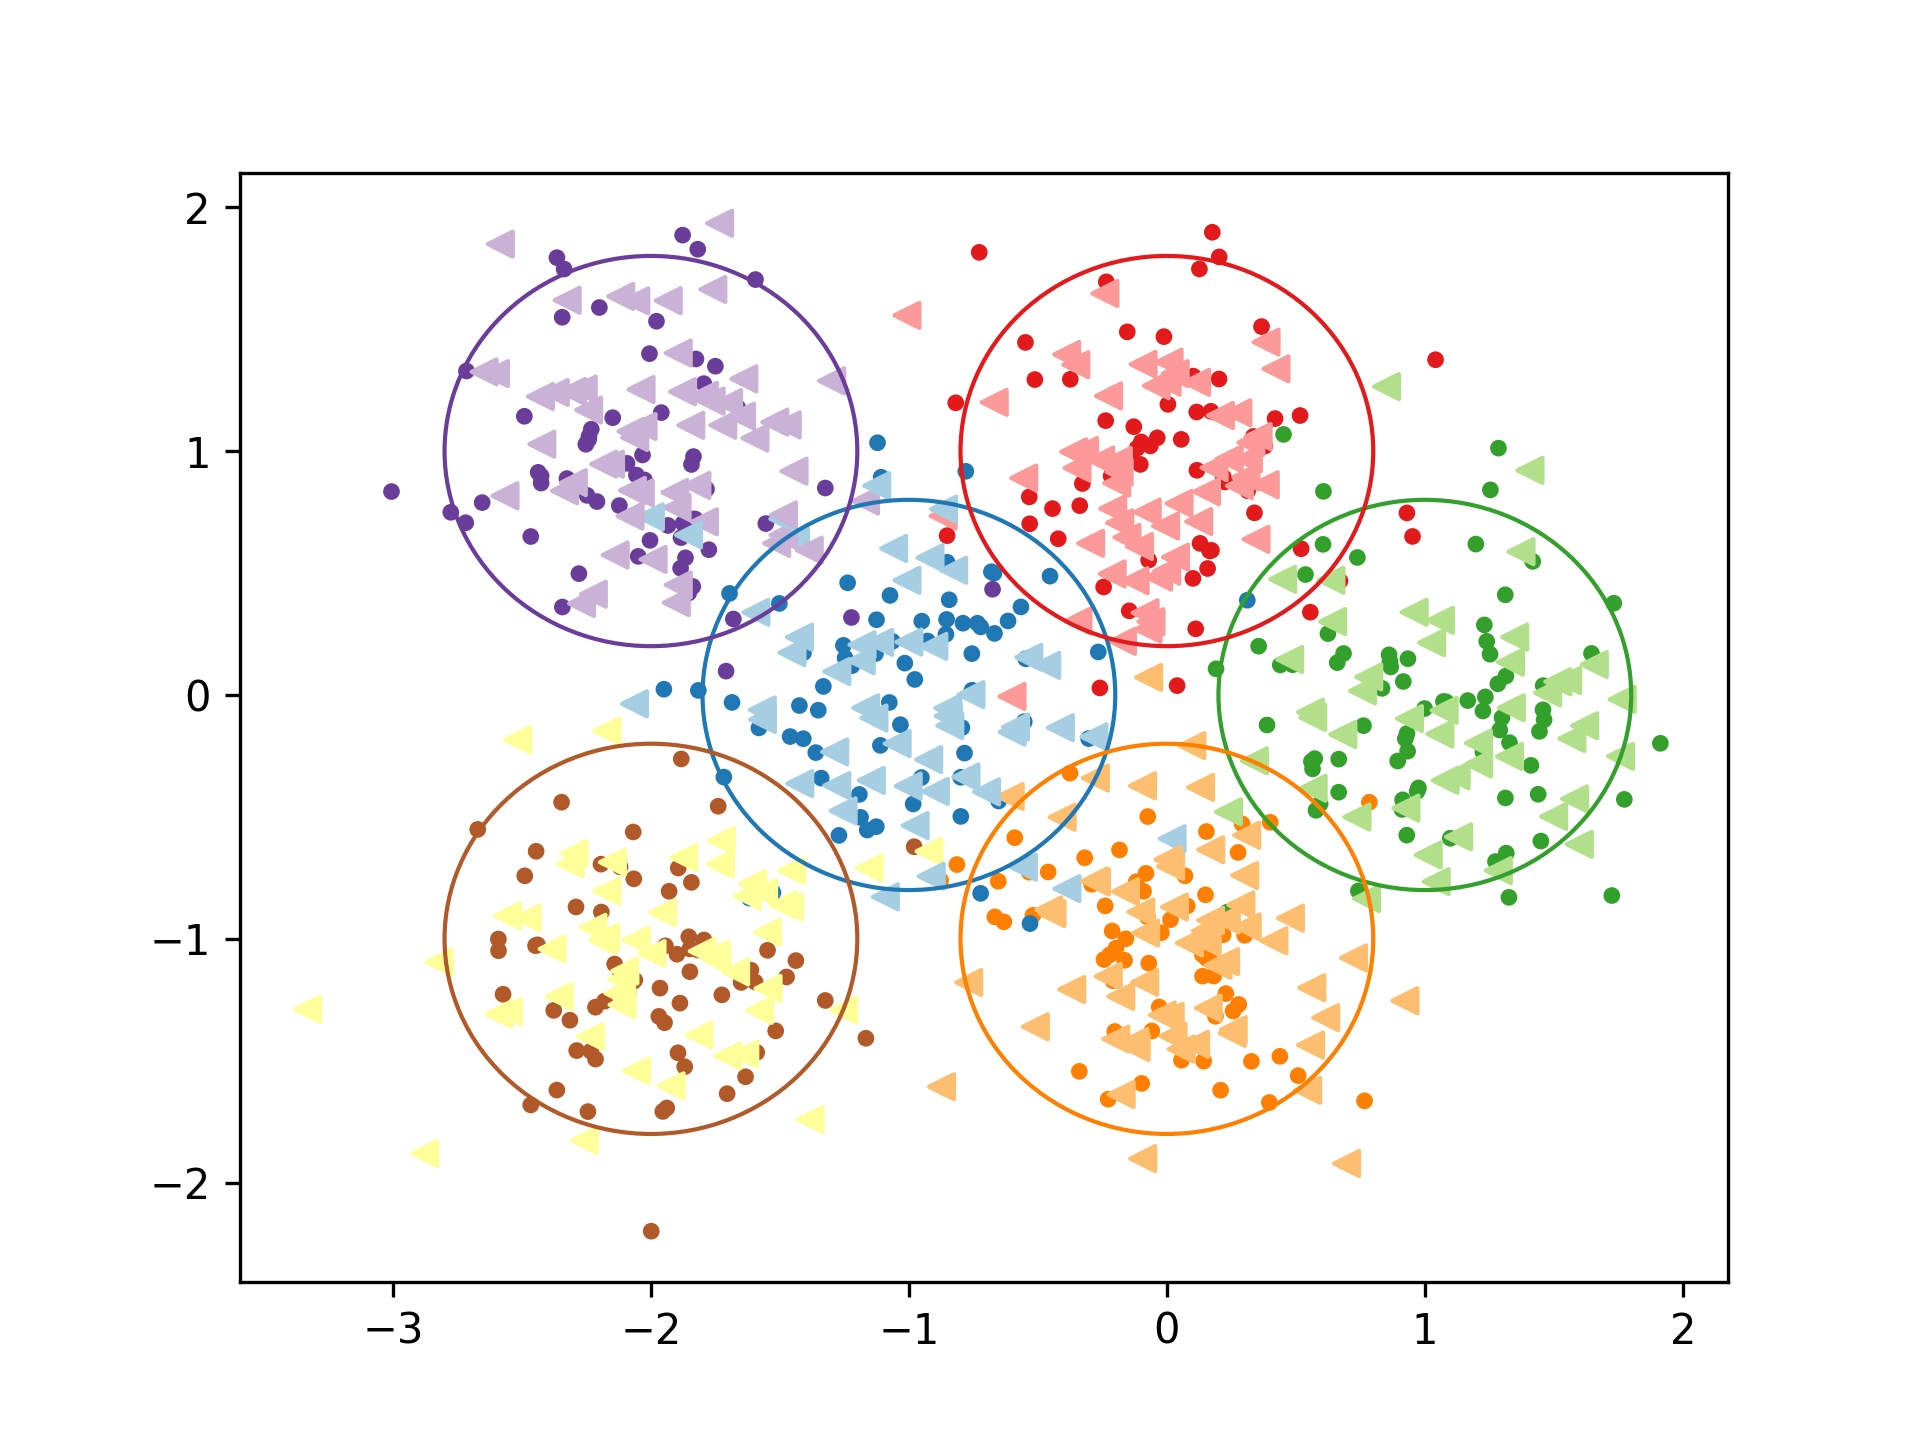
\includegraphics[width=0.7\textwidth]{./images/dataset.png}
    \caption{Ejemplo del \textit{dataset}}
    \label{fig:digitos}
\end{figure}

\begin{figure}[H]
    \centering
    \lstinputlisting[firstline=25,lastline=39, style=custompython]{../evaluation.py}
    \caption{Función \textit{generate\_data}}
    \label{fig:generate_data}
\end{figure}

\begin{figure}[H]
    \centering
    \lstinputlisting[firstline=288,lastline=308, style=custompython]{../evaluation.py}
    \caption{Función \textit{plot\_data}}
    \label{fig:plot_data}
\end{figure}

\begin{figure}[H]
    \centering
    \lstinputlisting[firstline=330,lastline=346, style=custompython]{../evaluation.py}
    \caption{Función \textit{generate\_data\_driver}}
    \label{fig:generate_data_driver}
\end{figure}

Una vez más haremos uso de la clase \textit{CommandLine} con nuevos argumentos para el uso concreto de este programa:

\begin{figure}[H]
    \centering
    \lstinputlisting[style=custompython]{../commandline.py}
    \caption{Clase \textit{CommandLine}}
    \label{fig:CommandLine}
\end{figure}

\section{Modelo complejo}

Usando \textit{pytorch} haremos un modelo complejo visto en la función \textit{ComplexModel()} (figura \ref{fig:ComplexModel}). Este modelo (y el resto) se componen usando la clase \textit{torch.nn.Sequential}. Las características de este modelo son:
\begin{itemize}
    \item Capa de 120 unidades y activación \textit{ReLu}
    \item Capa de 40 unidades y activación \textit{ReLu}
    \item Capa de 6 unidades y activación linear
\end{itemize}

Podemos ver los resultados en \textit{train} y \textit{cross-validation} en la figura \ref{fig:complex_results}. Para entrenar este modelo usaremos la función \textit{train\_model} (figura \ref{fig:train_model}) y las funciones \textit{train\_split} y \textit{train\_data}  (figuras \ref{fig:train_split} y \ref{fig:train_data})para preparar los datos para su procesado. Este modelo sobreajusta demasiado en datos de entrenamiento y falla en los datos de validación. Las funciones que llevan todo este proceso son \textit{complex\_model} y \textit{complex\_model\_driver} (figuras \ref{fig:complex_model} y \ref{fig:complex_model_driver}).

La función \textit{acc} nos dice si una predicción es acertada o no y \textit{evaluate\_model} nos da la precisión del modelo (figuras \ref{fig:acc} y \ref{fig:evaluate_model}), mientras que las funciones \textit{plot\_loss\_accuracy} y \textit{plot\_decision\_boundary} nos muestran la evolución de la precisión y la frontera de decisión respectivamente.

\begin{figure}[H]
    \centering
    \lstinputlisting[firstline=4,lastline=19, style=custompython]{../ComplexModel.py}
    \caption{Función \textit{ComplexModel}}
    \label{fig:ComplexModel}
\end{figure}

\begin{figure}[H]
    \centering
    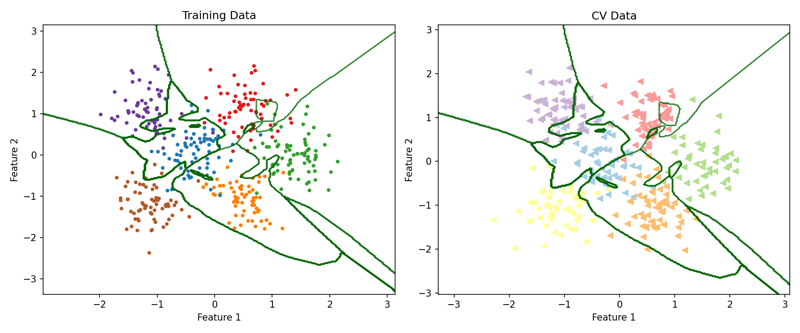
\includegraphics[width=0.7\textwidth]{./images/decision_boundary_complex.png}
    \caption{Resultados del modelo complejo}
\end{figure}

\begin{figure}[H]
    \centering
    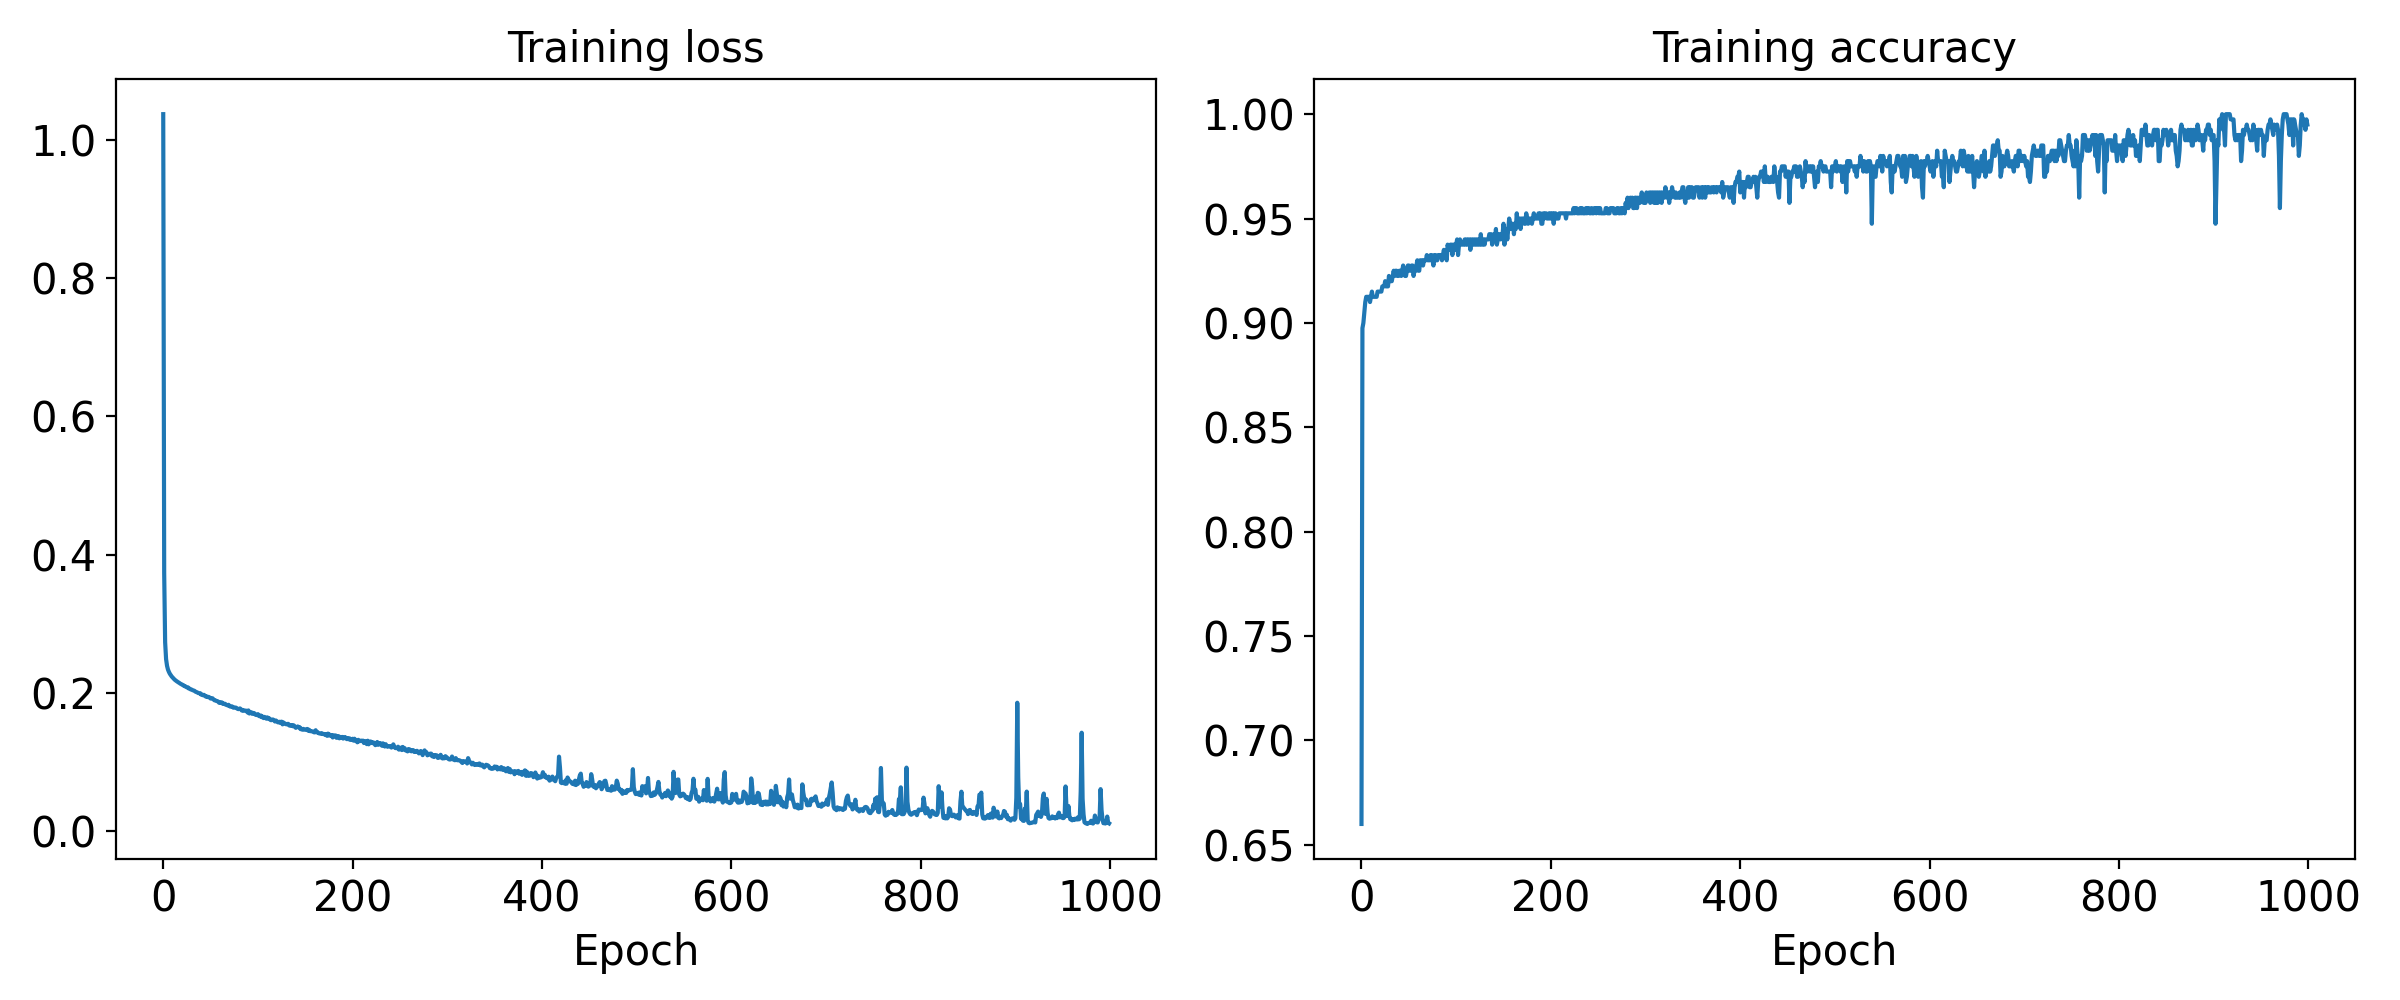
\includegraphics[width=0.7\textwidth]{./images/loss_accuracy_complex.png}
    \caption{Resultados del modelo complejo}
    \label{fig:complex_results}
\end{figure}


\begin{figure}[H]
    \centering
    \lstinputlisting[firstline=94,lastline=130, style=custompython]{../evaluation.py}
    \caption{Función \textit{train\_model}}
    \label{fig:train_model}
\end{figure}

\begin{figure}[H]
    \centering
    \lstinputlisting[firstline=42,lastline=54, style=custompython]{../evaluation.py}
    \caption{Función \textit{train\_split}}
    \label{fig:train_split}
\end{figure}

\begin{figure}[H]
    \centering
    \lstinputlisting[firstline=57,lastline=78, style=custompython]{../evaluation.py}
    \caption{Función \textit{train\_data}}
    \label{fig:train_data}
\end{figure}

\begin{figure}[H]
    \centering
    \lstinputlisting[firstline=133,lastline=154, style=custompython]{../evaluation.py}
    \caption{Función \textit{complex\_model}}
    \label{fig:complex_model}
\end{figure}

\begin{figure}[H]
    \centering
    \lstinputlisting[firstline=372,lastline=392, style=custompython]{../evaluation.py}
    \caption{Función \textit{complex\_model\_driver}}
    \label{fig:complex_model_driver}
\end{figure}

\begin{figure}[H]
    \centering
    \lstinputlisting[firstline=81,lastline=91, style=custompython]{../evaluation.py}
    \caption{Función \textit{acc}}
    \label{fig:acc}
\end{figure}

\begin{figure}[H]
    \centering
    \lstinputlisting[firstline=258,lastline=285, style=custompython]{../evaluation.py}
    \caption{Función \textit{evaluate\_model}}
    \label{fig:evaluate_model}
\end{figure}

\begin{figure}[H]
    \centering
    \lstinputlisting[firstline=203,lastline=224, style=custompython]{../evaluation.py}
    \caption{Función \textit{plot\_loss\_accuracy}}
    \label{fig:plot_loss_accuracy}
\end{figure}

\begin{figure}[H]
    \centering
    \lstinputlisting[firstline=227,lastline=255, style=custompython]{../evaluation.py}
    \caption{Función \textit{plot\_decision\_boundary}}
    \label{fig:plot_decision_boundary}
\end{figure}
\section{Modelo simple}

Usando \textit{pytorch} haremos un modelo simple visto en la función \textit{SimpleModel()} (figura \ref{fig:SimpleModel}). Las características de este modelo son:
\begin{itemize}
    \item Capa de 6 unidades y activación \textit{ReLu}
    \item Capa de 6 unidades y activación linear
\end{itemize}

Podemos ver los resultados en \textit{train} y \textit{cross-validation} en la figura \ref{fig:simple_results}. Para entrenar este modelo usaremos las funciones presentadas en el apartado anterior y las funciones \textit{simple\_model} y \textit{simple\_model\_driver}

\begin{figure}[H]
    \centering
    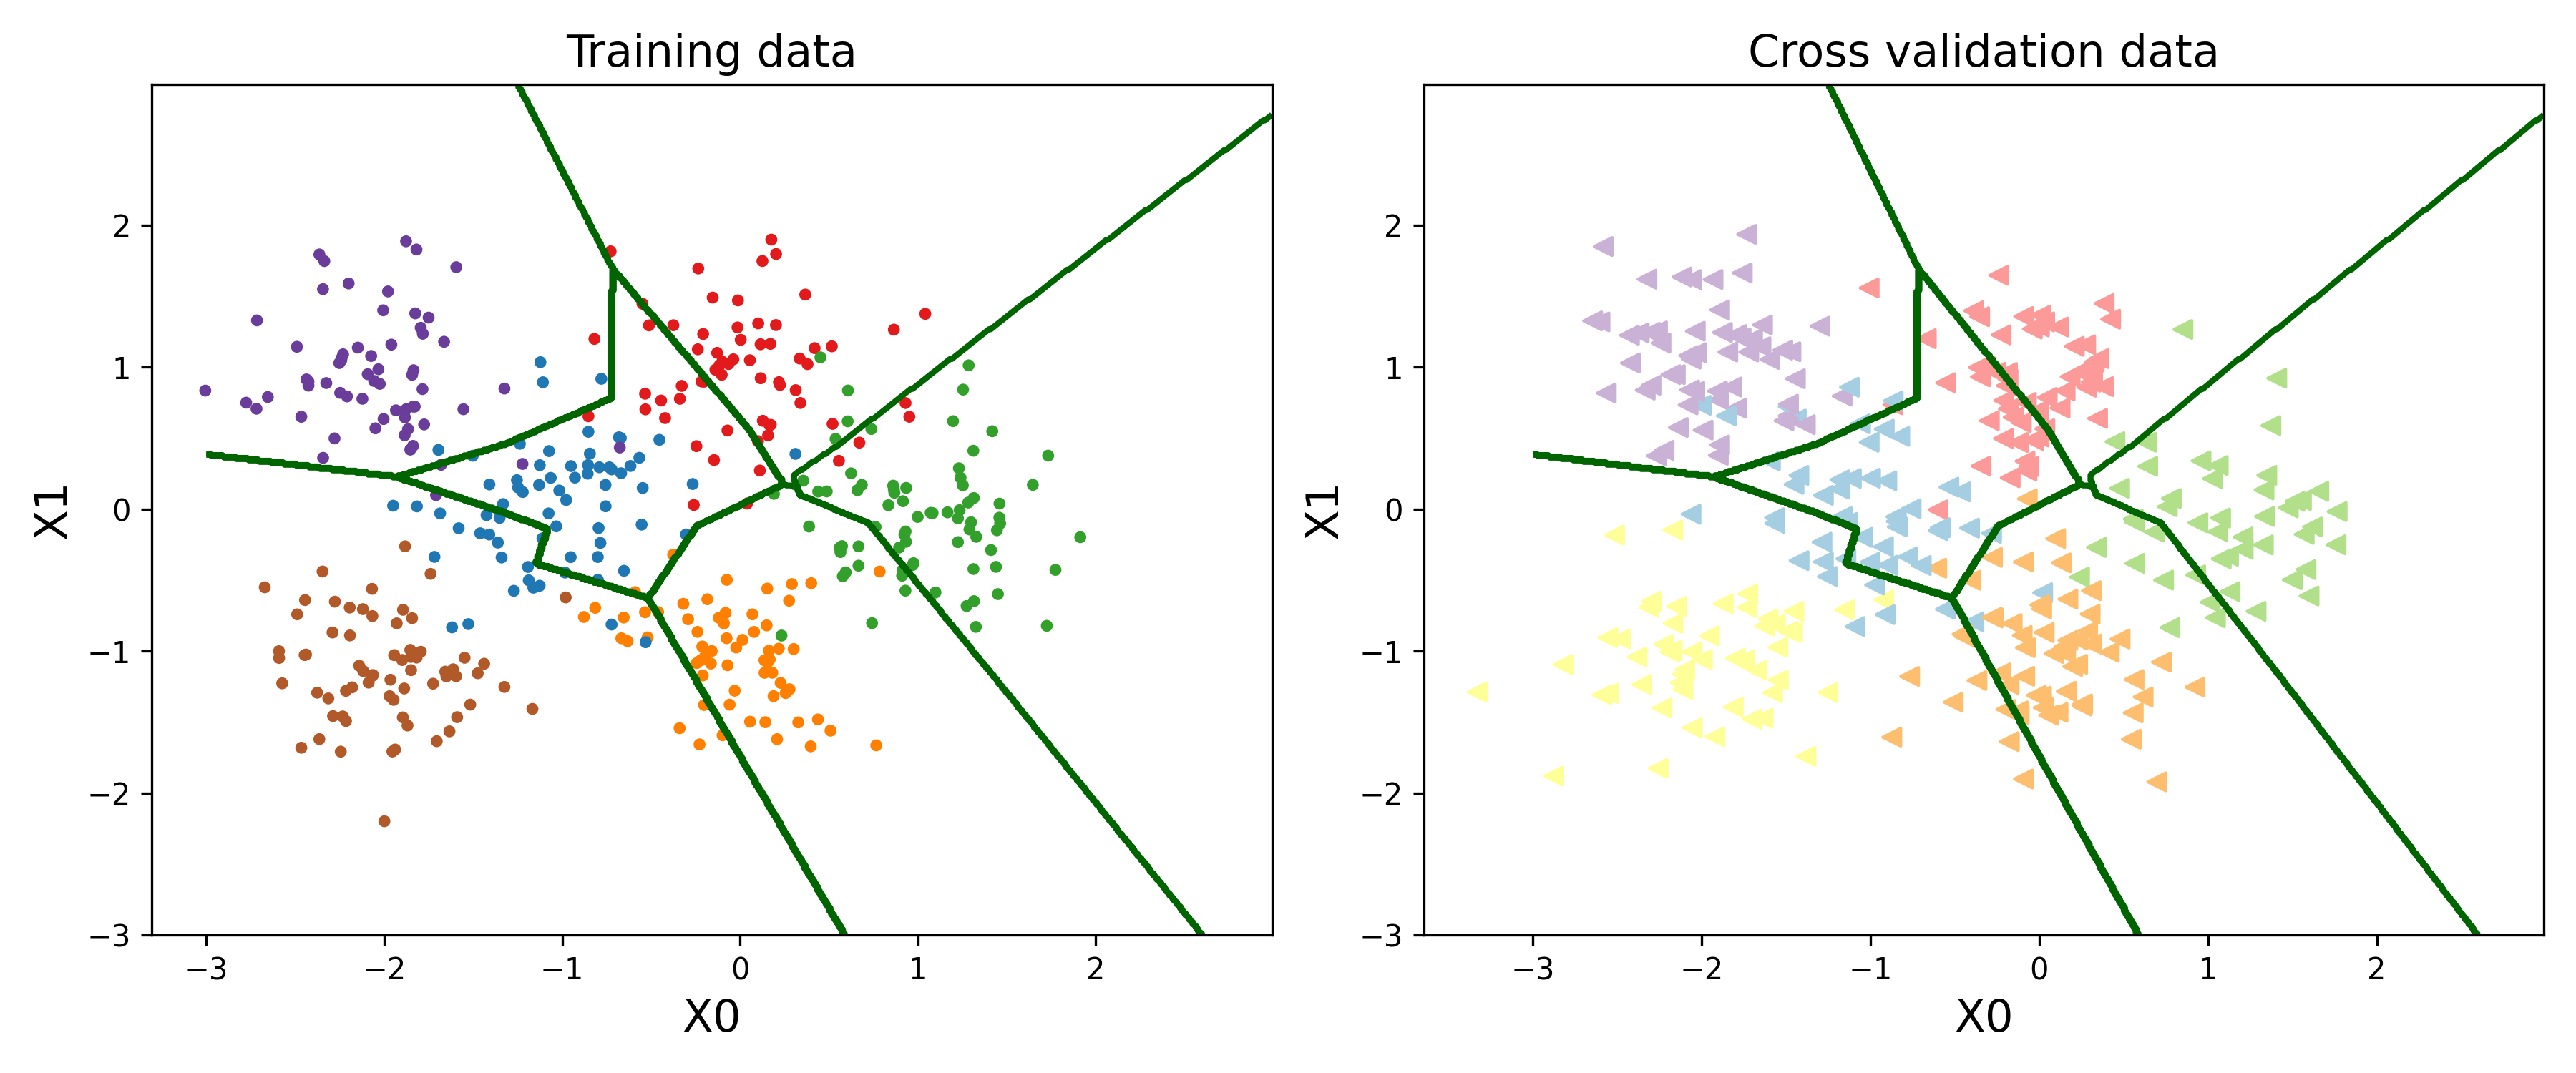
\includegraphics[width=0.7\textwidth]{./images/decision_boundary_simple.png}
    \caption{Resultados del modelo simple}
    \label{fig:simple_results}
\end{figure}

\begin{figure}[H]
    \centering
    \lstinputlisting[firstline=4,lastline=15, style=custompython]{../SimpleModel.py}
    \caption{Función \textit{SimpleModel}}
    \label{fig:SimpleModel}
\end{figure}

\begin{figure}[H]
    \centering
    \lstinputlisting[firstline=349,lastline=369, style=custompython]{../evaluation.py}
    \caption{Función \textit{simple\_model\_driver}}
    \label{fig:simple_model_driver}
\end{figure}

\begin{figure}[H]
    \centering
    \lstinputlisting[firstline=157,lastline=176, style=custompython]{../evaluation.py}
    \caption{Función \textit{simple\_model}}
    \label{fig:simple_model}
\end{figure}



\section{Modelo regularizado}

En este modelo usaremos el modelo del apartado 1. Las características de este modelo son:
\begin{itemize}
    \item Capa de 120 unidades y activación \textit{ReLu}
    \item Capa de 40 unidades y activación \textit{ReLu}
    \item Capa de 6 unidades y activación linear
\end{itemize}

Para regularizar este modelo usaremos la función \textit{train\_model} (figura \ref{fig:train_model}). Podemos ver los resultados en \textit{train} y \textit{cross-validation} en la figura \ref{fig:regularized_results}. Las funciones que llevan todo este proceso son \textit{regularized\_model} y \textit{regularized\_model\_driver}.


\begin{figure}[H]
    \centering
    \lstinputlisting[firstline=179,lastline=200, style=custompython]{../evaluation.py}
    \caption{Función \textit{regularized\_model}}
    \label{fig:regularized_model}
\end{figure}

\begin{figure}[H]
    \centering
    \lstinputlisting[firstline=395,lastline=416, style=custompython]{../evaluation.py}
    \caption{Función \textit{regularized\_model\_driver}}
    \label{fig:regularized_model_driver}
\end{figure}

\begin{figure}[H]
    \centering
    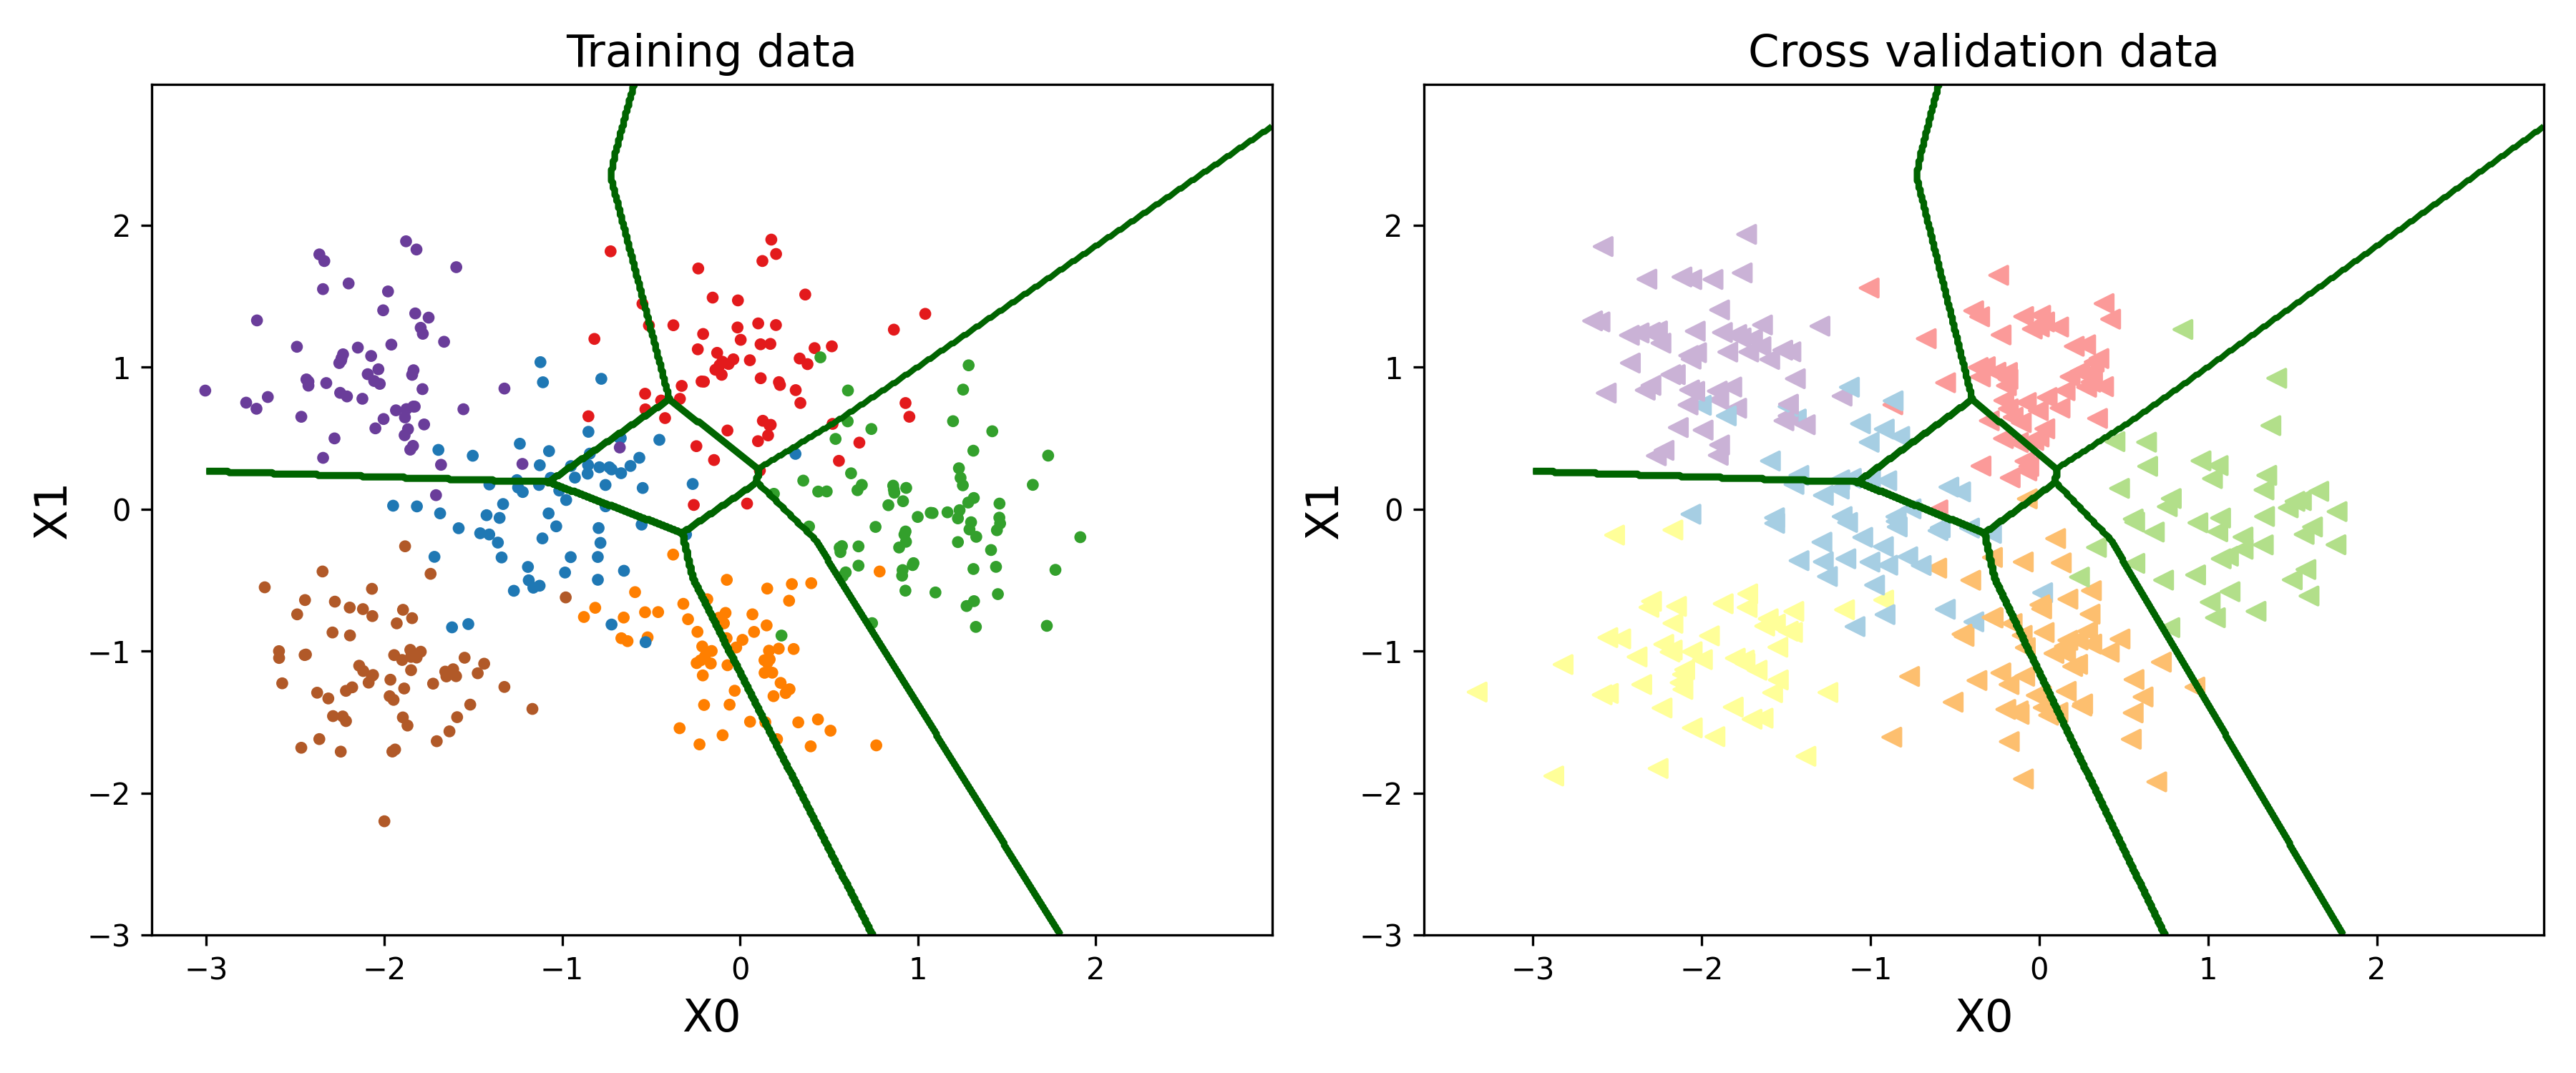
\includegraphics[width=0.7\textwidth]{./images/decision_boundary_regularized.png}
    \caption{Modelo regularizado}
    \label{fig:regularized_results}
\end{figure}



\section{Elegir el valor de regularización}

Usando el sistema del modelo regularizado, vamos a escoger el mejor $\lambda$ para regularizar el modelo. Para ello usaremos la función \textit{reg\_test\_driver} (figura \ref{fig:reg_test_driver}). Podemos ver los resultados en la figura \ref{fig:lambda_results}. La función que genera este gráfico es \textit{plot\_regularization} (figura \ref{fig:plot_regularization}).

Obtenemos que el mejor valor de $\lambda$ es 0.01. Podemos ver el modelo regularizado en la imagen \ref{fig:optim_res}.

\begin{figure}[H]
    \centering
    \lstinputlisting[firstline=419,lastline=444, style=custompython]{../evaluation.py}
    \caption{Función \textit{reg\_test\_driver}}
    \label{fig:reg_test_driver}
\end{figure}

\begin{figure}[H]
    \centering
    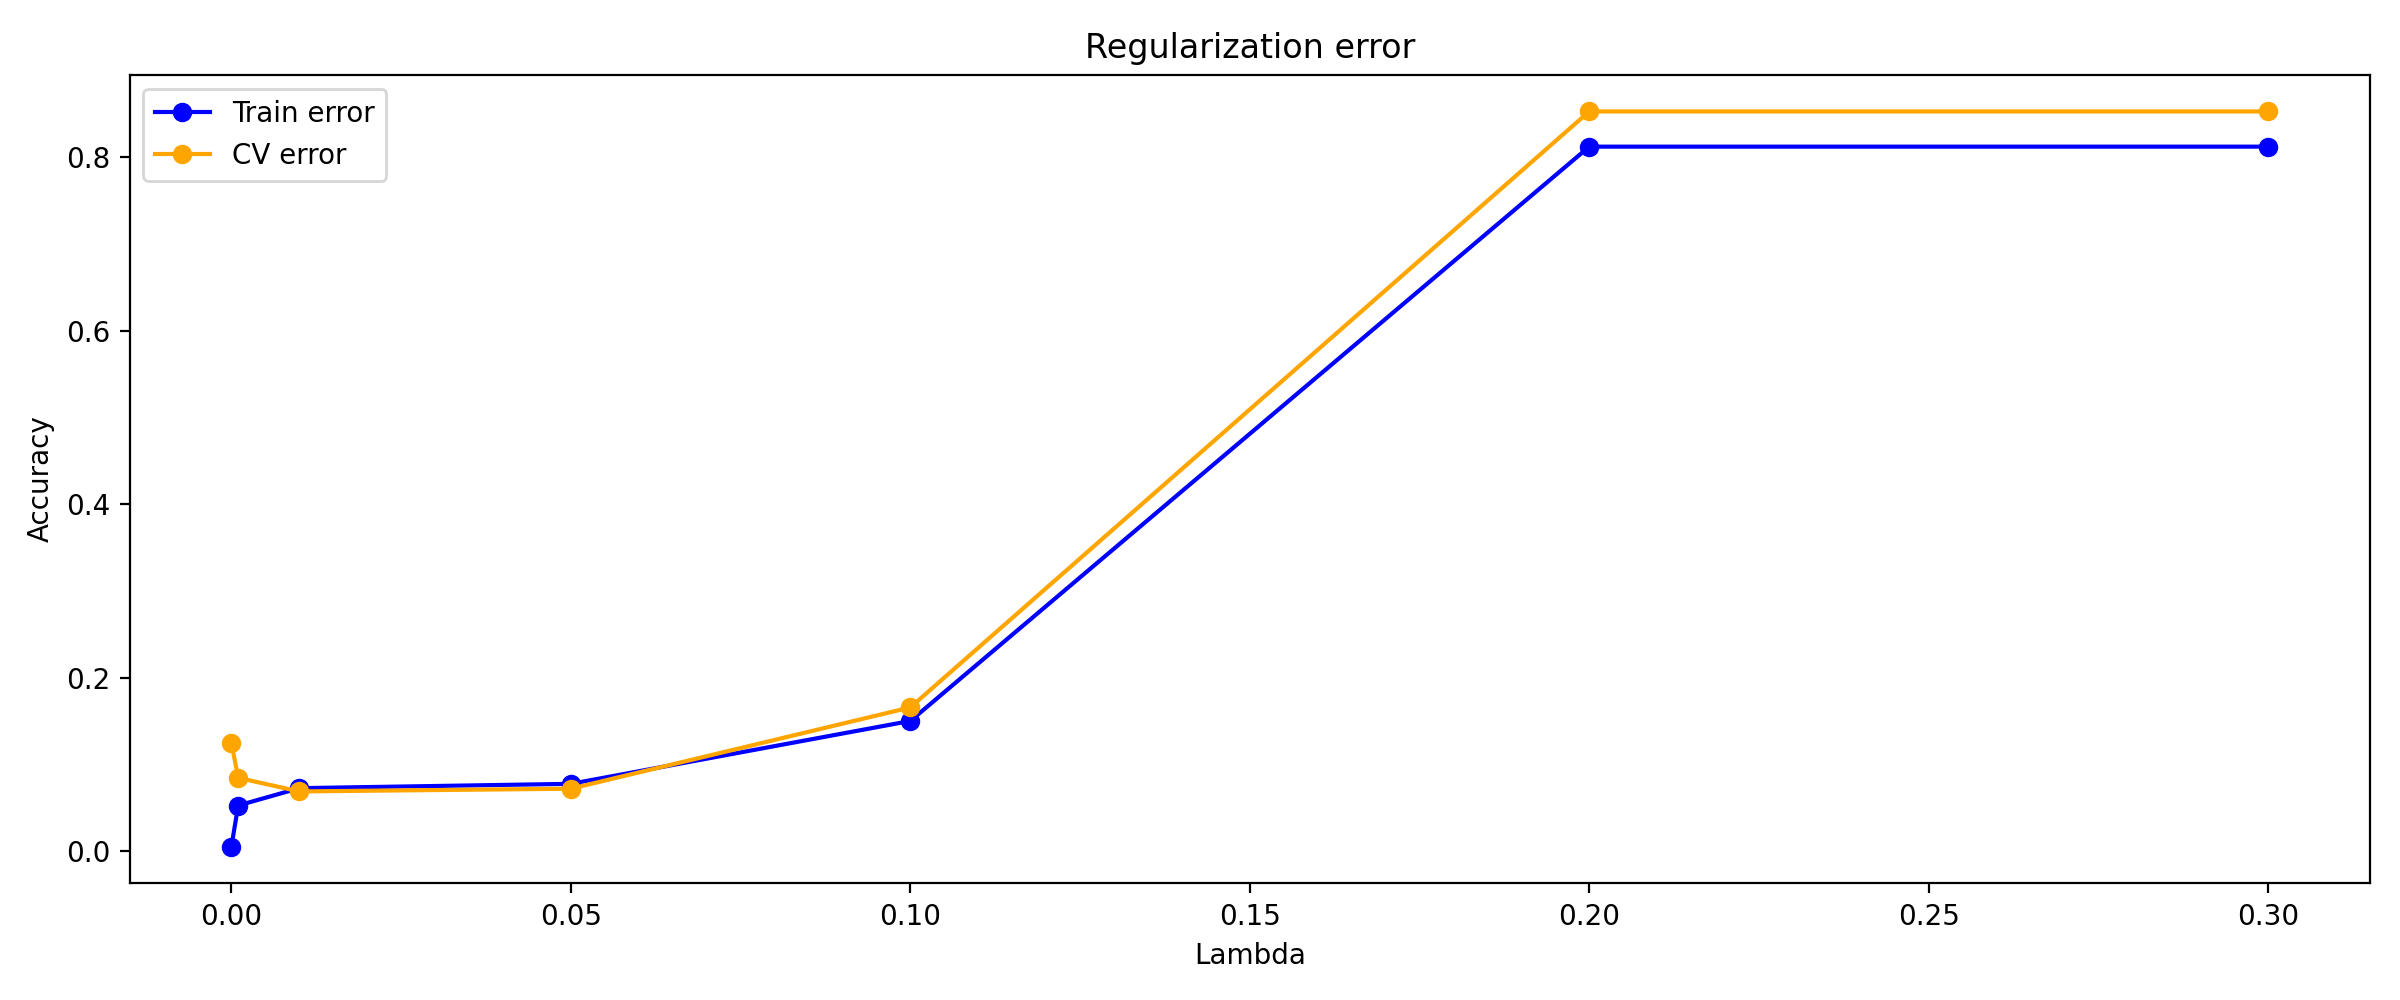
\includegraphics[width=0.7\textwidth]{./images/tuning.png}
    \caption{Resultados de la regularización}
    \label{fig:lambda_results}
\end{figure}

\begin{figure}[H]
    \centering
    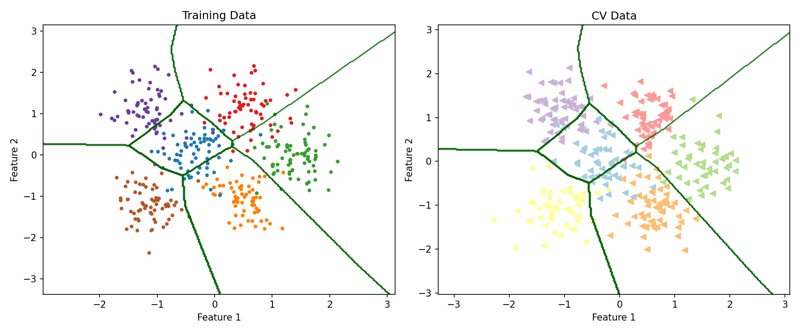
\includegraphics[width=0.7\textwidth]{./images/decision_boundary_regularized_optimal.png}
    \caption{Modelo óptimo}
    \label{fig:optim_res}
\end{figure}

\begin{figure}[H]
    \centering
    \lstinputlisting[firstline=311,lastline=327, style=custompython]{../evaluation.py}
    \caption{Función \textit{plot\_regularization}}
    \label{fig:plot_regularization}
\end{figure}



\end{document}
